\documentclass[svgnames,dvipsnames,hyperref={bookmarks=false},usepdftitle=false]{beamer}
\usetheme{scalameta}

\title{scala.meta}
\subtitle{Semester projects for Spring 2015}
\author{Eugene Burmako (\href{https://twitter.com/xeno_by}{@xeno{\textunderscore}by})}
\institute{\'Ecole Polytechnique F\'ed\'erale de Lausanne \\ \texttt{http://scalameta.org/}}
\date{26 November 2014}
\hypersetup{pdfauthor={Eugene Burmako},pdftitle={Semester projects for Spring 2015}}

\begin{document}

\titleframe

\sectionframe{What do we do?}

\begin{frame}{Metaprogramming is...}
\begin{quote}
Metaprogramming is the writing of computer programs that write or manipulate other programs or themselves as their data.
\end{quote}
\begin{flushright}
\textemdash Wikipedia
\end{flushright}
\end{frame}

\begin{frame}{Notable metaprograms}
\begin{itemize}
\item Compilers
\item Code generators
\item IDEs
\end{itemize}
\end{frame}

\begin{frame}[c, fragile]{Before Scala 2.10}
\begin{center}
% http://completenostalgia.com/transport/
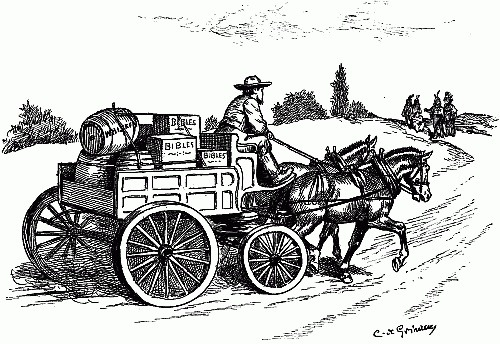
\includegraphics[height=7cm]{horse.jpg}
\end{center}
\end{frame}

\begin{frame}[c, fragile]{We are building a better tech}
\begin{center}
% http://www.utopiaplanitia.info/blueprints.html
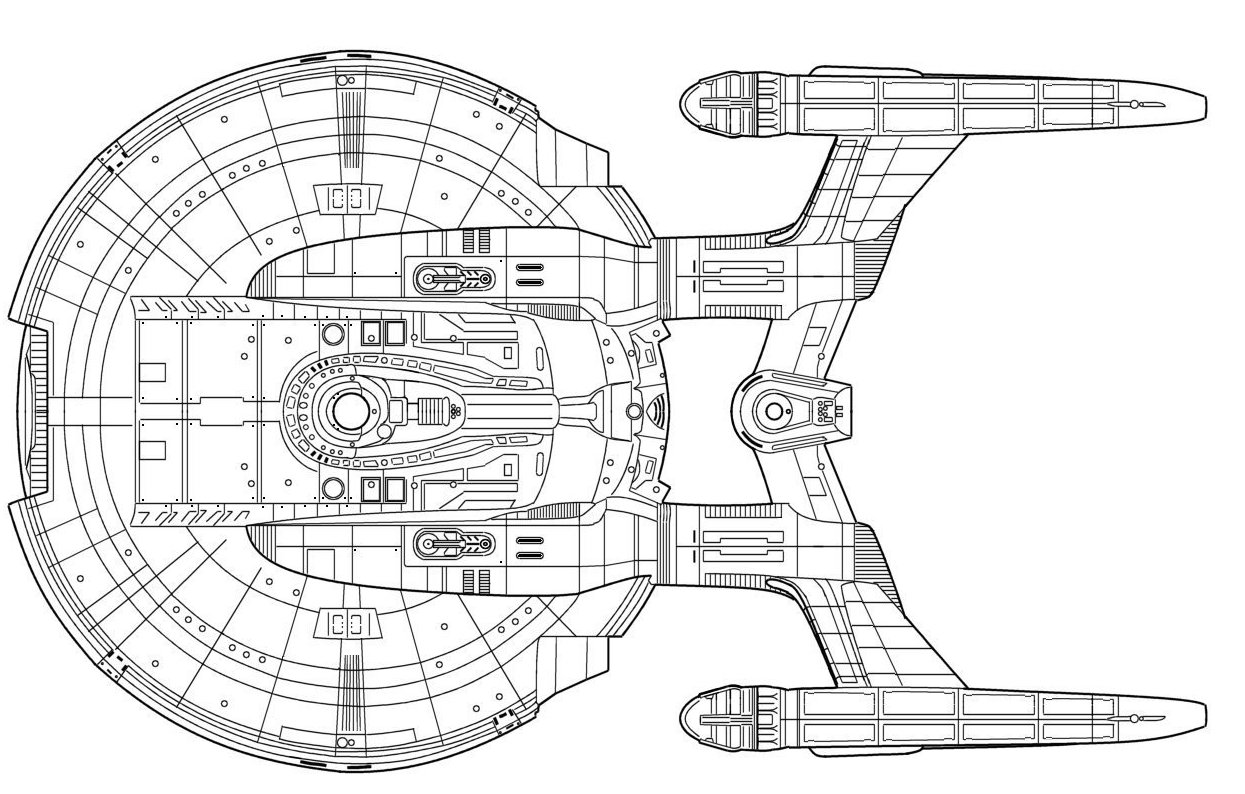
\includegraphics[height=7.5cm]{nx01-wireframe.jpg}
\end{center}
\end{frame}

\sectionframe{Why would you care?}

\begin{frame}[fragile, t]
\frametitle{Reason \#1: Innovate in programming languages}

\begin{semiverbatim}
val usersMatching = query[String, (Int, String)](
  "select id, name from users where name = ?")
usersMatching("John")

\only<2->{case class User(id: Column[Int], name: Column[String])}
\only<2->{users.filter(_.name === "John")}

\only<3->{case class User(id: Int, name: String)}
\only<3->{users\alert{.filter(}_.name == "John"\alert{)}}

\end{semiverbatim}

\begin{itemize}
\item Database queries can be written in SQL
\only<2->{\item They can also be written in a DSL, at times slightly awkward}
\only<3->{\item Or they can be written in Scala and virtualized by a macro}
\end{itemize}
\end{frame}

\begin{frame}[fragile]
\frametitle{Reason \#1: Innovate in programming languages}

\begin{semiverbatim}
trait Query[T] \{
  \alert{def filter(p: T => Boolean): Query[T] = macro ...}
\}

val users: Query[User] = ...
users\alert{.filter(}_.name == "John"\alert{)}


                          \arrowdown

Query(Filter(users, Equals(Ref("name"), Literal("John"))))

\end{semiverbatim}

\begin{itemize}
\item The \texttt{filter} macro takes an AST corresponding to the predicate
\item This AST is then analyzed and transformed into a query fragment
\item \alert{C\# and F\# need dedicated language features for this, we don't!}
\end{itemize}
\end{frame}

\begin{frame}[fragile]{Reason \#2: Implement stuff that people will use}
\begin{semiverbatim}
ClassDef(
  NoMods,
  newTypeName("D"),
  Nil,
  Template(
    List(Ident(newTypeName("C"))),
    emptyValDef,
    List(DefDef(NoMods, nme.CONSTRUCTOR, ...))))

\end{semiverbatim}
\begin{itemize}
\item Once, the most reliable way to do ASTs was via vanilla datatypes
\item Above you can see what it took to say \texttt{class D extends C}
\item Needless to say, only brave souls cared to use such an API
\end{itemize}
\end{frame}

\begin{frame}[fragile]{Reason \#2: Implement stuff that people will use}
\begin{semiverbatim}
val tree = q"class D extends C"
val q"class \$_ extends ..\$parents" = tree

\end{semiverbatim}
\begin{itemize}
\item Then we introduced quasiquotes, a template-based approach to ASTs
\item They became wildly popular even before an official release
\item And the biggest features of Scala 2.11
\item \alert{A fun fact: quasiquotes were a semester project at LAMP.\\ Thanks, Denys, for your hard work!}
\end{itemize}
\end{frame}

\begin{frame}{Reason \#2: Implement stuff that people will use}
\begin{itemize}
\item Another great example is work done by Martin Duhem
\item When he started tinkering with SBT, macro support was pretty subpar
\item \alert{A couple months in, Martin managed to make things much better and his improvements were already included in SBT 0.13.5}
\end{itemize}
\end{frame}

\begin{frame}{Reason \#3: Influence future developments in Scala}
\begin{itemize}
\item AST persistence was once a cute little idea
\item We saw and appreciated its potential and decided to dig in
\item Of course, as a semester project here at LAMP!
\end{itemize}
\end{frame}

\begin{frame}{Reason \#3: Influence future developments in Scala}
\begin{itemize}
\item Adrien Ghosn \& Mathieu Demarne approached the project in a very creative way
\item \alert{Thanks to awesome prototype and great presentation, they've managed to convince people that AST persistence is practical}
\item The seeds were planted, and in the autumn we had a breakthrough!
\end{itemize}
\end{frame}

\begin{frame}[c, fragile]{Reason \#3: Influence future developments in Scala}
\begin{center}
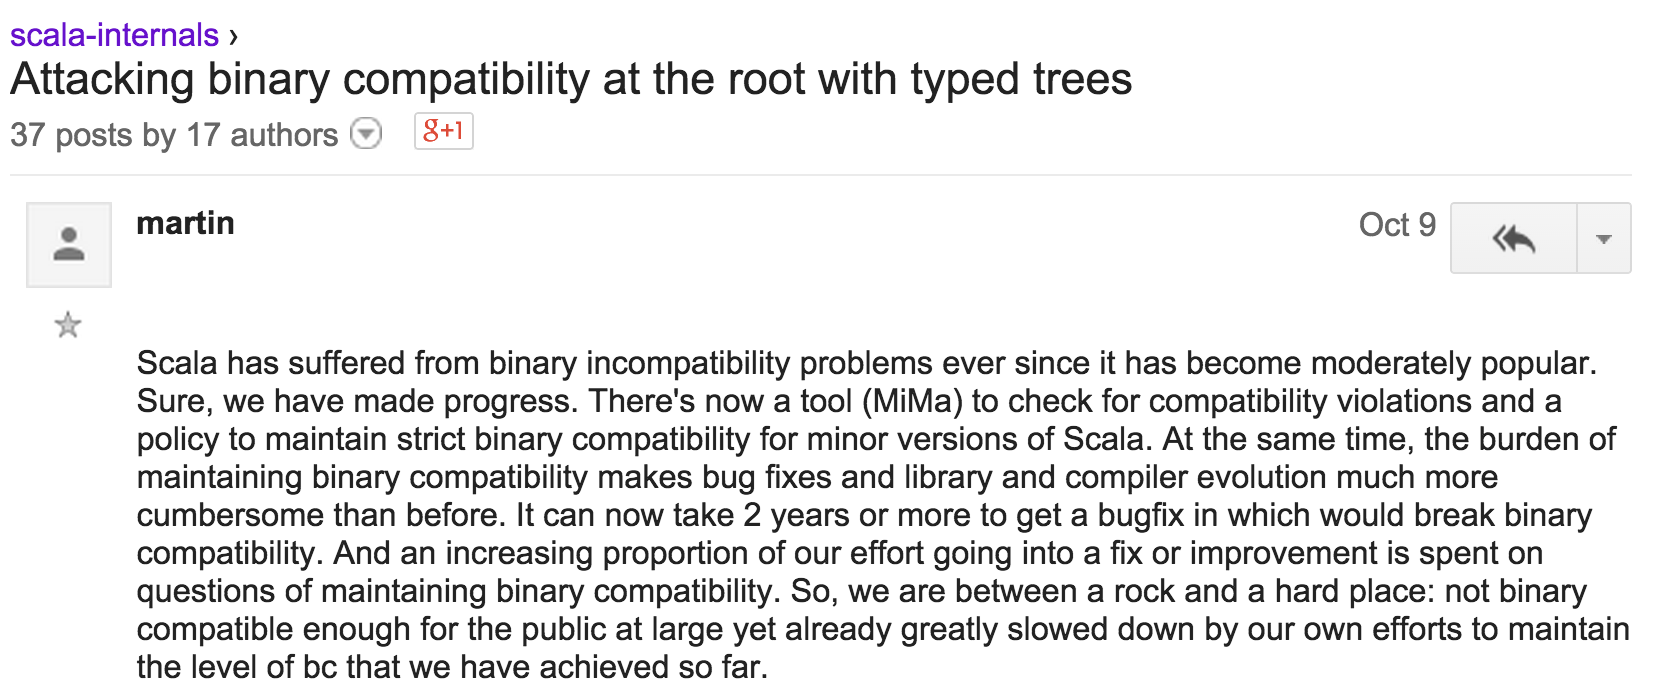
\includegraphics[height=5cm]{martin.png}
\end{center}
\end{frame}

\sectionframe{What projects do we have?}

\begin{frame}{Summary}
\begin{itemize}
\item Obey: linter \& migrator
\item Metadoc: a nextgen doc tool
\item IDE support for debugging metaprograms
\item A new and improved parser for Scala
\end{itemize}
\end{frame}

\end{document}